\indent Rekapitulasi tersebut diurutkan berdasarkan besarnya/signifikansi persentase perbedaan antara kedua platform, dapat dilihat pada Tabel \ref{user-test-recap-sorted}.
\LTXtable{\textwidth}{table/05/pengguna/recap_sorted}

Visualisasi perbandingan dapat dilihat lewat diagram garis pada Gambar \ref{diagram-pengguna-chart}.

\begin{figure}[H]
	\centering
	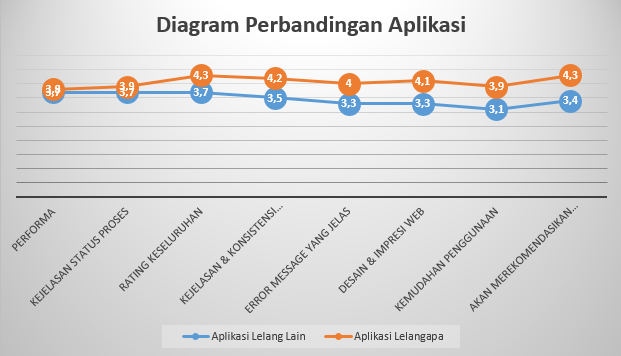
\includegraphics[width=\textwidth]{images/bab5/ujipengguna/chart.png}
	\caption{Diagram Perbandingan Pengujian \textit{User Experience} Pengguna}
	\label{diagram-pengguna-chart}
\end{figure}

\newpage
Dalam hal ini, dapat disimpulkan bahwa impresi \textit{user experience} sudah baik, dan skor \textit{user experience}nya sedikit diatas sistem serupa lainnya. Perbedaannya sudah cukup signifikan adalah \textit{recommendation}, kemudahan penggunaan dan desain \textit{web} yang baik. Namun, yang menjadi perhatian adalah perbedaan \textit{performa} yang masih sangat kecil. Hal ini terkait dengan pengujian \textit{speed test} di subbab selanjutnya.